\documentclass[12pt,a4paper]{article}
\usepackage[bottom=2.5cm,top=3.5cm]{geometry}
%\usepackage{ngerman}
\usepackage[utf8]{inputenc}
\usepackage[T1]{fontenc}
\usepackage{microtype}
\usepackage{graphics}
\usepackage{ae}
\usepackage{amssymb}
\usepackage{amsmath}
\usepackage{amsthm}
\usepackage[margin=10pt,font=small,labelfont=bf]{caption}
%\usepackage[pdftex]{graphicx}
\usepackage{listings}
%\linespread{1.25}
\setlength{\parindent}{0pt}

\usepackage{fancyhdr}
\usepackage[
  	pdfstartview=FitH,   
  	pdffitwindow=true,
	pdftitle = "Optimisation SS10 UdS", % Sets the document information Title field
    pdfauthor = "Adrian Neumann and Sebastion Steenbruck", %Sets the document information Author field
  	colorlinks,
  	linkcolor=black,
  	anchorcolor=black,
  	citecolor=black,
  	urlcolor=black
]{hyperref}

\pagestyle{fancy}
\cfoot{\thepage}
\rfoot{
\includegraphics{./images/by-nc-sa.pdf}}
\fancyhead{}
\lfoot{}
\renewcommand{\footrulewidth}{0.4pt}
\renewcommand{\headrulewidth}{0pt}
\newcommand{\N}[0]{\mathbb{N}}
\newcommand{\Z}[0]{\mathbb{Z}}
\newcommand{\Q}[0]{\mathbb{Q}}
\newcommand{\R}[0]{\mathbb{R}}
\newcommand{\C}[0]{\mathbb{C}}
\newcommand{\im}[0]{\mathit{i}}
\newcommand{\nthings}[1]{{#1}_1,\ldots,{#1}_n}
\newcommand{\norm}[1]{|\!|#1|\!|}
\newtheoremstyle{leplain} %name
    {3pt} %above
    {3pt} %below
    {} %body font
    {} %indent
    {\bfseries} %head font
    {:} %punctuation after head
    {0.5em} %space after head
    {} %head spec
\title{Optimisation}
\author{Adrian Neumann \\ {\small \texttt{adrian\_neumann@gmx.de}} \and Sebastian Steenbuck \\ {\small\texttt{sebastian@steenbuck.org}}}
\date{}\begin{document}
\lstset{language=Java, basicstyle=\ttfamily\small\upshape, commentstyle=\slshape\sffamily, keywordstyle=\em, breaklines=true}

\theoremstyle{definition}
\newtheorem{Def}{Definition}

\theoremstyle{leplain}
\newtheorem{Ex}{Example}
\newtheorem{pr}{Proof}

\theoremstyle{theorem}
\newtheorem{thm}{Theorem}



\maketitle
\thispagestyle{fancy}

\marginpar{Tutorial}
\section*{Tutorial}
Some definitions from linear algebra, which were repeated in the tutorial.

Linear algebra was originally developed from geometry but has come to be an important foundation in mathematics. To keep things simple we'll restrict ourselves to $\R^n$ although other structures could be used.

\begin{Def}[Vector space] 
A vector space (for our purposes) is a set of points $$\R^n=\{(x_1,x_2,...,x_n)|x_i \in \R\}$$ that is closed under linear combination.
\end{Def}

\begin{Def}[Linear Combination] 
A linear combination $w$ is defined as the sum of all the vectors in a set $V$ multiplied with some scalars $\lambda$.
$$w=\sum_{i \in V}{\lambda_i v_i} \qquad \lambda_i \in \R,v_i\in V$$ 
\end{Def}  

As infinite sets are hard to describe we're looking for a \emph{Basis} $S$. Which is a subset of $\R^n$ such that every vector in $\R^n$ can be represented as a unique linear combination of the elements of $S$.

The vectors in a basis must be \emph{linearly independent}, that is none of them can be written as a linear combination of the others. The standard basis for $\R^n$ is the set of $n$-dimensional unit vectors.

\[\left\{\begin{pmatrix}1\\0\\\vdots\\0\end{pmatrix},\begin{pmatrix}0\\1\\\vdots\\0\end{pmatrix},\ldots,\begin{pmatrix}0\\\vdots\\0\\1\end{pmatrix}\right\}\]


\begin{thm} 
Every basis of a vector space $\R^n$ has the same number of elements, which is $n$. 
\end{thm}

This follows for example from \href{http://en.wikipedia.org/wiki/Steinitz_exchange_lemma}{Steinitz exchange lemma}.

\begin{Def}[Subspace]
 A subspace $V$ of a vector space $\R^n$ is spanned by a subset of the a basis of $R^n$. Examples of a subspace in 2D are all the lines going through the point $(0,0) \in \R^2$.
\end{Def}

To get a notion of angle between vectors we introduce the dot product (in euclidean spaces also called: inner product). It is defined as

\[\langle x,y\rangle  = \sum x_iy_i\]

It is related to the law of cosines in two dimensions ($c^2 = a^2+b^2-2ab\cos \gamma$) like this:

\begin{minipage}[hbt]{0.5\linewidth}
\begin{align*}
\norm{\vec c}^2 &= \norm{\vec a}^2 + \norm{\vec b}^2 -2\norm{\vec a}\norm{\vec b}\cos \gamma\\
\norm{a-b}^2 &= \norm{\vec a}^2 + \norm{\vec b}^2 -2\norm{\vec a}\norm{\vec b}\cos \gamma\\
\norm{a}^2-2\langle a,b\rangle +\norm{b}^2 &= \norm{\vec a}^2 + \norm{\vec b}^2 -2\norm{\vec a}\norm{\vec b}\cos \gamma\\
\frac{\langle a,b\rangle }{\norm{a}\norm{b}} = \cos \gamma
\end{align*}
\end{minipage}
\hfill
\begin{minipage}[hbt]{0.3\linewidth}
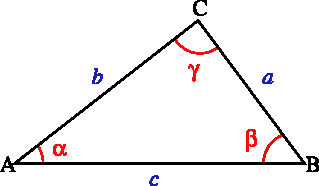
\includegraphics[scale=0.8]{./images/Triangle_with_notations_2.pdf}
\end{minipage}

\bigskip
(Here $\norm{a}$ denotes the norm: $\sqrt{\sum a_i^2} = \sqrt{\langle a,a\rangle }$). The dot product is $0$ if and only if the vectors are orthogonal to each other.

Now that we have defined vector spaces we want to study some linear transformations on them. Since vector spaces are closed under linear combination we'd like to have our transformation preserve that structure.

\begin{Def}[Linear Transformation] A linear transformation is (for our purposes) a mapping $T : \R^n \rightarrow \R^m$ with the following properties:

\begin{enumerate}
\item $T(\lambda w) = \lambda T(w)$
\item $T(v+w) = T(v)+T(w)$
\end{enumerate}
\end{Def}

Prominent examples for linear transformations are rotations and reflections around the origin. Note that if $T(\vec 0)\neq 0$ you automatically know that it's not a linear transformation.

If we use a standard basis for our vector space we can easily represent linear transformations by their effects on the basis. Just map every basis vector to its image and write the results in a matrix. 

\begin{Ex}[Reflection] Suppose we want to reflect every vector in $\R^2$ at the x-axis. If we use the standard base $V = \{(1,0),(0,1)\}$ and compute its reflection $V'=\{(1,0),(0,-1)\}$ we get the matrix

\[R = \begin{pmatrix}
1 & 0 \\
0 & -1
\end{pmatrix}\]

Multiplying a vector with that matrix we get its reflection. Just in case: Matrix multiplication

\[\begin{pmatrix}
a_{11} & a_{12} & \ldots & a_{1n}\\
a_{21} & a_{22} & \ldots & a_{2n}\\
\vdots \\
a_{m1} & a_{m2} & \ldots & a_{mn}
\end{pmatrix} * \begin{pmatrix}x_1\\x_2\\\vdots\\x_n\end{pmatrix} =\begin{pmatrix} \sum_{i=1}^n a_{1i}x_i\\ \sum_{i=1}^n a_{2i}x_i\\\vdots\\\sum_{i=1}^n a_{mi}x_i\end{pmatrix}\]

\end{Ex}

Note that for two transformations $f,g$ and their matrices $A,B$ we have
\[\forall \vec v:\ (f\circ g)(v) = (AB)v\]

\begin{Def}[Kernel of a matrix] 
 The kernel of a matrix $A$ is the set of all vectors $x$ with
$$Ax=0$$
\end{Def}

\begin{Def}[Rank of a matrix]
 The rank of a matrix $A$ is the number of linearly independent columns or rows of $A$. The column and row rank is always the same. In other words the row (column) rank is the dimension of the subspace spanned by the rows of $A$. A matrix $A^{m \times n}$ is said to have a full rank if $rank(A)=min(m,n)$
\end{Def}

If a matrix $A$ has full rank its kernel has dimension 0 and any system of equations $A x=b$ has a unique solution $A^{-1}b$. You can invert such matrices for example by using a Gauss-Jordan elimination. If the matrix is sparse it may be faster to calculate the inverse by

\[A^{-1} = \frac{1}{\det A} \tilde A \qquad \tilde a_{ij} = (-1)^{i+j} \det A_{ji}\]

Where $A_{ji}$ is the matrix $A$ without the $i$-th row and the $j$-th column and $\det A$ is the determinant of the matrix. It can be computed recursively:

\[\det A = \sum_{i=1}^n a_{ij} \cdot (-1)^{i+j} \det A_{ij} = \sum_{j=1}^n a_{ij} \cdot (-1)^{i+j} \det A_{ij} \]

For example
\[\det \begin{pmatrix} 
3 & 9 & 1\\
2 & 5 & 4\\
-2 & 8 & 7\end{pmatrix} \stackrel{i=2}{=}
-2\cdot \det \underbrace{\begin{pmatrix} 
9 & 1\\ 
8 & 7\end{pmatrix}}_{A_{21}} + 
5\cdot \det \underbrace{\begin{pmatrix}
3 & 1\\
-2 & 7\end{pmatrix}}_{A_{22}} -
4\cdot \det \underbrace{\begin{pmatrix} 
3 & 9\\ 
-2 & 8\end{pmatrix}}_{A_{23}}= -163\]

Here we fixed the second row and iterated over the columns. Since we multiply by $a_{ij}$ in each recursion step this procedure is fast if there are lots of zeros in the matrix.

\marginpar{Lecture 1}
\section{Introduction and Examples}
\marginpar{Lecture 2}
\section{Solving Linear Programs}
A linear program in general has the form:
\begin{eqnarray*}
\text{minimize:}& \vec c \cdot \vec x \\
\text{subject to:} & A \cdot \vec x \geq \vec b
\end{eqnarray*}
$x=\{x_1,x_2,..,x_n\}$ is an vector of variables in $\R$. $x$ together with the vector $c \in \R^n$ is the objective function.
$A^{m \times n}$ together with $x\in \R^m$ and $b \in \R^m$is the system of inequation which describes the constrains.
%From now on we'll characterize the system of inequation by a matrix and a vector. $A\vec x \geq \vec b$. The objective function can also be written in vector form $\min \vec c \vec x$, where $c$ is the cost vector.

Solving LPs with just two variables is rather easy. We can use a graphical approach in two dimensions. The constraints define halfplanes in the 2D space. The feasible region of the problem is then the intersection of all the halfplanes. The cost vector now defines a halfspace of its own (i.e. lines with equivalent costs) that can be shifted around by choosing different $x$. If $x$ lies within the feasible region we get a feasible solution. The goal is to shift the lines as far in negative $c$ direction as possible without leaving the feasible region. See figure \ref{Fig:graphSolutionEx}.

\begin{figure}[hbt]
\begin{minipage}[hbt]{0.4\linewidth}
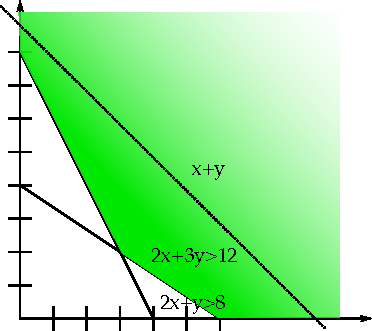
\includegraphics{./images/graphSolutionEx.pdf}
\end{minipage}
\hfill
\begin{minipage}[hbt]{0.4\linewidth}
\begin{align*}
\min x+y\\
2x+y\geq 8\\
2x+3y\geq 12
\end{align*}
\end{minipage}
\caption{An example for a graphical solution of an LP. The optimal solution is (3,2)}
\label{Fig:graphSolutionEx}
\end{figure}

How can we derive an algorithm from this method? We use the idea of sliding down, but just look at the corners of the feasible region, to get discrete steps (continuous sliding can't be implemented well). We start with any corner of the feasible region (a basic feasible solution) and look at its neighbors. Should they have a better objective value we move, else we're finished. 

To formalize the intuition from the 2D-space we need a notion of a corner in a (usually high dimensional) feasible region. To use it in a algorithm it should be a non-graphical definition. First we give some general definitions and then three different alternative definitions of a corner. We finish by proving that they are all equivalent.

\begin{Def}[Polyhedron] A set in $\R^n$ whose members obey a set of linear inequalities
\[\{x\in \R^n | Ax \geq b\} \qquad A\in \R^{m\times n},\ b\in \R^m\]
\end{Def}

\begin{Def}[Hyperplane, Hyperspace] \label{Def:hyperPlaneSpace} Let $a,x\in \R^n$, $a\neq 0$. 
\begin{enumerate}
\item $\{x|ax=b\}$ is a \emph{hyperplane} (a line in 2D)
\item $\{x|ax\geq b\}$ is a \emph{halfspace} (halfplane in 2D)
\end{enumerate}
\end{Def}

With definition \ref{Def:hyperPlaneSpace} we can say that a polyhedron is an intersection of a bunch of halfspaces.

\begin{Def}[Convex Sets] A subset $S \subseteq \R^n$ is called \emph{convex} if any convex combination between two points (graphically: points on a line between those points) is contained in the set. See figure \ref{Fig:convexNotConvex}
\[\forall \lambda \in [0,1], \forall x,y\in S: \lambda x + (1-\lambda) y \in S\]
\end{Def}

\begin{figure}[hbt]
\begin{center}
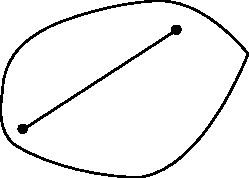
\includegraphics{./images/convex.pdf}\hspace{2cm}

\includegraphics{./images/notConvex.pdf}
\end{center}
\caption{Graphical example for a convex and a non convex set (with non linear borders)}
\label{Fig:convexNotConvex}
\end{figure}

Convex sets have a lot of nice properties. Luckily feasible regions are always convex. This is the main reason why we can efficiently solve LPs. 

\subsection*{Corners}
The following three definitions formalize the notion of a corner.

\begin{Def}[Vertex]\label{Def:Vertex} Let P be a polyhedron. A vector $x\in P$ is a \emph{vertex} of P if $\exists \vec c\in \R^n$
 s.t. $cx < cy$ for all $y\in P, y \neq x $; that is $x$ is the minimal point for some cost vector (the unique optimal solution for some LP with the feasible set P). See figure \ref{Fig:vertex}
\end{Def}

\begin{figure}[hbt]
\begin{center}
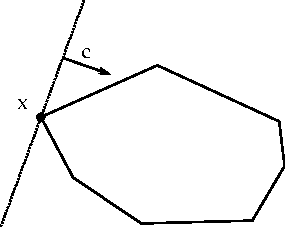
\includegraphics{./images/vertex.pdf}
\end{center}
\caption{A vertex $x$ is the optimal solution for a cost vector $c$}
\label{Fig:vertex}
\end{figure}

\begin{Def}[Extreme Point]\label{Def:ExtremePoint} An \emph{extreme point} of a polyhedron P is a vector $x\in P$ s.t. $x$ is not a convex combination of any two vectors $y,z\in P$ different from $x$. 
\end{Def}
Example: In 2D we can always select the two adjacent corners of a point $x$ on the edge of $P$ iff $x$ is not a corner. Then $x$ will be on the line between the two corners. 

\begin{Def}[Active Constraint]\label{Def:ActiveConstraint} Let $P$ be a polyhedron that is defined by some linear inequalities $a_i$: $P=\{x|a_ix\geq b_i\}$. We'll say that the $i$-th constraint is \emph{active} at a point $x$ if we have equality there $a_ix = b_i$
\end{Def}

\begin{Def}[Basic Feasible Solution]\label{Def:BFS} Let $P$ be a polyhedron in $n$ dimensions. Then $x\in P$ is a \emph{basic feasible solution} if the set of active constraints has full rank, that is there are $n$ linearly independent active constraint vectors at the point $x$. See figure \ref{Fig:bfsActiveConstraints}
\[\mbox{rank}(\{a_i\in \R^n|a_ix=b_i\}) = n\]

In particular there never is a b.f.s. if we have less than $n$ constraints. (Example: A line in 2D-Space or a plane in 3D-Space)
\end{Def}

\begin{figure}[hbt]
\begin{center}
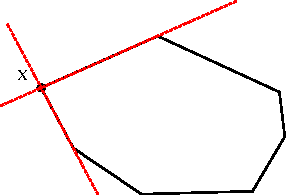
\includegraphics{./images/bfs.pdf}
\end{center}
\caption{Two constraints (red lines) are active at $x$. It's a basic feasible solution}
\label{Fig:bfsActiveConstraints}
\end{figure}

Now we want to prove that the three definitions \ref{Def:Vertex}, \ref{Def:ExtremePoint} and \ref{Def:BFS} are all equivalent to each other.

\begin{thm} \label{Thm:cornerEquiv} Let $P$ be a polyhedron and $x\in P$. The following are equivalent
\begin{enumerate}
\item $x$ is a vertex
\item $x$ is an extreme point
\item $x$ is a basic feasible solution
\end{enumerate}
\end{thm}

\begin{pr}[Theorem \ref{Thm:cornerEquiv}] The proof goes in three steps
\begin{itemize}
\item vertex $\Rightarrow$ extreme point: Proof by contraposition. Assume the existence of $y,z \in P$ s.t. $y,z\neq x$ with $x= \lambda y + (1-\lambda )z$. That is, $x$ is not an extreme point (definition \ref{Def:ExtremePoint}). We want to show that it's not a vertex either.

From definition a vertex (def. \ref{Def:Vertex}) we know that some $c$ should exist such that $c x < c \lambda y  + c (1-\lambda) z$. That however is a contradiction to the assumption $x= \lambda y + (1-\lambda )z$.
\begin{align*}
cx &= \lambda cy +(1-\lambda)cz\\
   &< \lambda cx + (1-\lambda)cx\\
   &< cx
\end{align*}

\item extreme point $\Rightarrow$ bsf (proof by contraposition; we show $\neg \text{bsf} \Rightarrow \neg \text{extreme point}$): Suppose $x\in P$ is not a basic feasible solution. Let $B$ be a matrix of active constraints at $x$ and $C$ the matrix of the inactive constraints such that $Bx=d$, $Cx\gneq f$ and $A = \left[B\atop C\right]$. Since $x$ is not a bfs the matrix $B$ hasn't full rank and its kernel is nonempty. Hence

\[\exists \delta \in \R^n, \delta \neq 0:\ B\delta =0\]

See figure \ref{Fig:extremeBfs}. With $\delta$ we define two vectors:

\[y=x+\epsilon \delta \quad z = x-\epsilon \delta\]

Note that $x=(z+y)/2$. That means that $x$ is not an extreme point if $z,y \in P$, because $x$ is a convex combination of the two. Consider 

\[Bz = B(x+\epsilon \delta) = Bx + \epsilon B\delta = Bx\]

Since $B\delta = 0$ the active constraints are still active. For the inactive constraints we have some slack before we leave the polyhedron (We can move around on the red line in figure \ref{Fig:extremeBfs}). If we choose $\epsilon$ small enough we're still within. It suffices to choose $\epsilon$ such that 

\[\forall i: \epsilon |c_i z| < c_i x - f_i\qquad \vec c_i\in C,\ f_i \in \vec f\]

Hence $z$ (and analogous $y$) are still in the polyhedron and $x$ is not an extreme point.

\begin{figure}
\begin{center}
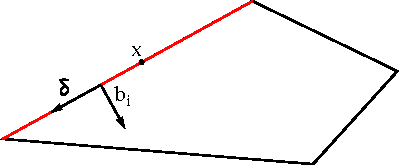
\includegraphics{./images/extreme_bfs.pdf}
\end{center}
\caption{$x$, active constraint $b_i$ and orthogonal vector $\delta$}
\label{Fig:extremeBfs}
\end{figure}

\item bfs $\Rightarrow$ vertex: Suppose $x$ is a bsf. Let $I$ be the indices of all active constraints and $c=\sum_{i \in I} a_i$. Then $c x = \sum_{i \in I} b_i$, since for each $a_i x \geq b_i $ the inequality is tight (see def. \ref{Def:ActiveConstraint}). 

Also $\forall y\in P, i\in I$ we have $a_i y \geq b_i$. Therefore $c y \geq c x$. The greater then is sharp as $x$ is the unique solution to the active constraints because it's a bfs and the system of active constraints has full rank, i.e. if n-lines cross in n-dimensional space they do so at \emph{one} point. (Theorem 2.2 in the Linear Optimization book). So $x$ is the optimal solution for some LP and hence a vertex.
\end{itemize}

\subsection*{Standard Form}
A LP in standard form\footnote{Cormen et al. name this slack-form (Schlupfform)} is of the form:
\begin{eqnarray*}
\text{minimize:}& \vec c \cdot \vec x \\
\text{subject to:} & A \cdot \vec x = \vec b \\
& x\geq0
\end{eqnarray*}

Any LP can be transformed into an equivalent LP in standard form. Two steps are needed for this, one to add non negativity constraints for all variables and a second to transform any inequalities into a equalities.

\paragraph*{Add non negativity constraints:} Suppose a variable $x$ has no non-negativity constraint. $x$ can be replaced with two variables $x'$ and $x''$ such that $x=x'-x''$ and $x',x''\geq 0$, as any negative number can be written as a combination of two non negative numbers.

\paragraph*{Remove inequalities:} Suppose a constraint $a$ to be $x_1+2x_2 \geq 15$. By adding a new variable $s\in \R$ and the constraint $a-s=15$ we can remove the inequality. So by adding a new vector $s\in \R^n$ with $A \cdot \vec x - s = \vec b$ the inequalities can be removed.

\end{pr}

\end{document}
